\section{Evaluation}
\label{sec:eval}
We measured our DNS rebinding attack by two primary factors. We analyzed the \emph{time-to-launch} and the \emph{impact} of the attack. We then compared it to other two DNS rebinding mechanisms. 

\subsection{Time-to-Launch}
To protect from a time-varying attack that is able to establish an interactive session between the malicious server and the broswer, most modern browers have implemented DNS pinning that pin a DNS record for a period of time. At this time, a time-varying attack would take ~160 seconds to launch according to our experiment on the latest Chrome browser. However, by flooding the DNS table, we found that in the current Chrome implementation, if a DNS record is kicked out from the cache, the pinning time would dramatically decrease. We found that in our attack, only ~10 seconds is needed to launch the attack on a browser that have a cache size of 100 entries. 

In early 2013, the Chromium community has increased the size of DNS cache from 100 to 1000. This was not the result of security concerns, but rather a performance related patch. We then ran our experiments on the staging version Chrome, and found that it would only take 10 more seconds to flood the DNS table and launch the attack. 

Another approach of DNS rebinding is based on multiple A records attack. This attack needs only a small amount of time due to the number of packets transmitted, however this attack has certain limitations, we will discuss it in the next subsection.

\subsection{Impact}
We now evaluate the impact of our attack against other DNS rebinding approaches. As mentioned in the last section, the multiple A record approach has the advantage of requiring less time to launch. However, it has several limitations on its impact. First, the rebound IP address cannot be an internal IP address. Otherwise, the browser will prioritize it and select it in the first place which results in a failure to execute DNS rebinding. Second, the attacker cannot change the rebound IP address on the fly, which makes it unable to scan the subnet. 

For time-varying attack, although it is possible to bind to an internal IP address, it is also hard to change the rebound IP address on the fly due to the extremly long launching time. 

In our experiement, we are able to use FireDrill to rebind the domain name to an internal IP address to build a interactive session. Also, we are able to dynamically change the IP address during an attack. The attacker has the ability to navigate through the entire subnet instead of just one single IP address.

\subsection{Making The Victim Stay}
Our attack needs the victim's browser to act as a proxy. Thus it requires the victim to stay in the page for the attacker to have access to it. In order to do that, we designed a ``pending download`` page \ref{fig:download} that ask the victim to stay in the page for two minutes to download a file. While the victim is waiting for the download countdown, the JavaScript proxy is actually running in the background for the attacker to navigate through the internal websites. While it is often challenging to convince a user to stay on a website for such a long duration, we show that some scenarios facilitate such a requirement.

\begin{figure}[h]
\centering

\includegraphics[width=0.8\columnwidth]{download.png}
\caption{\textbf{Attack page.} The page that a victim first connects to. The user believes he is waiting for a file download to start on a free file-hosting website. While waiting for the file to be downloaded, the JavaScript is running in the the background as a proxy.}
\label{fig:download}
\end{figure}

\subsection{Changing the Content of Internal Wiki}
Now we demonstrate how to use FireDrill to access a victim's internal wiki. Many organizations have internal Wikis that contains extremly sensitive information and is only accessible through the company's local network or VPN. By building a session using the employee's browser as a proxy, the attacker could not only gain full access to the company's Wiki, but also the ability to change the content of it. Moreover, the modifications are done using the victim's IP address, adding to the anonymity of the attack, as shown in Figure \ref{fig:oldrevisions} In a real-world scenario, the attacker could potentially add malicious links into the Wiki in order to launch subsequent attacks.

\begin{figure}[h]
\centering
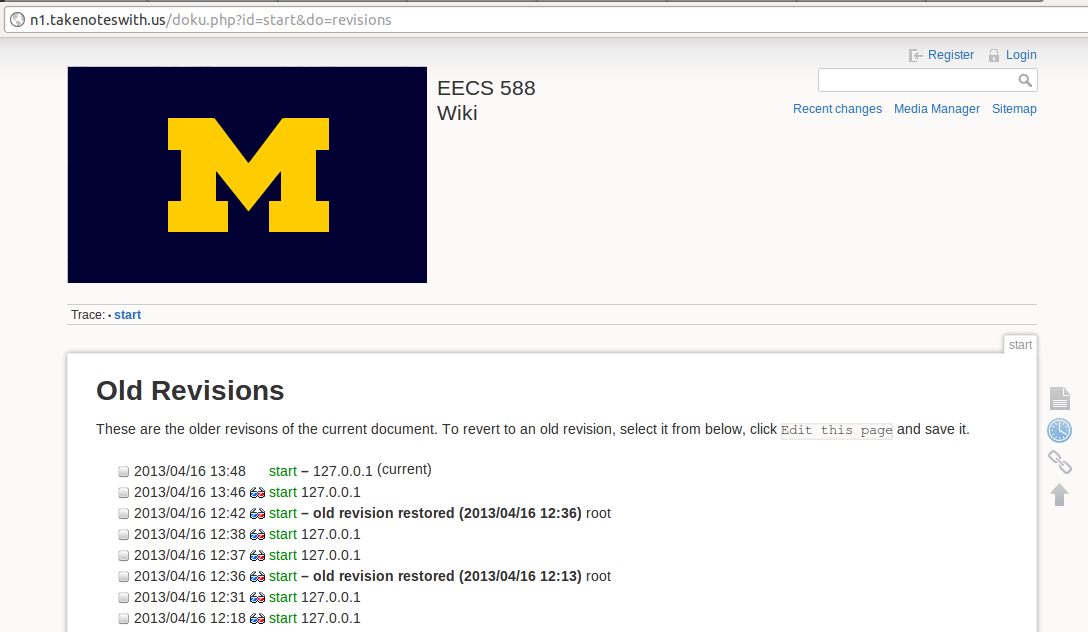
\includegraphics[width=0.8\columnwidth]{oldrevisions.png}
\caption{\textbf{Victim's web site's revision history.} The attacker can change the content of the company wiki anonymously. the revision history shows that the author of change was the victim's local IP address.}
\label{fig:oldrevisions}
\end{figure}

